\documentclass[12pt]{ctexart}

\usepackage{geometry}
\usepackage{indentfirst}
\usepackage{amsmath}
\usepackage{minibox}
\usepackage{graphicx}
\usepackage{subcaption}
\usepackage[export]{adjustbox}
\usepackage{float}
\usepackage{wrapfig}
\usepackage{amssymb}
\usepackage[framed,numbered,autolinebreaks,useliterate]{mcode}
\usepackage[utf8]{inputenc}
\usepackage[T1]{fontenc}

\geometry{top=1in,bottom=1in,left=0.5in,right=0.5in}

\title{Project 1 实验报告}
\author{缪方然}
\date{\today}

\begin{document}

\maketitle


\section{技术性实验}

\subsection{问题 1}

两种方法都\textbf{不}符合在单位圆中随机取点。

第一种方法的思路是先取定 $x$ 轴,再在 $[-\sqrt{1-x^2},\sqrt{1-x^2}]$ 之间取值,并记为 $y$。

第二种方法则是先选定半径 $r$ 的随机值,且在 \([0,1]\) 之间,之后在 $[0,2\pi]$ 之间选定辐角值,这样就可以得出 $x$,$y$ 的坐标了。

下面用数学实验与理论并行的方法来论证我的观点。

首先,在理想情况下,确定两个随机变量 $x$ 和 $y$ ,则他们服从

\[f(x,y)=\frac1{\pi},0\le x^2+y^2\le 1\]

$(x,y)$ 的均值为 $(0,0)$ ,而他们的协方差矩阵为

\[E\{[\mathbf X-E(\mathbf X)][\mathbf X-E(\mathbf X)]'\}
    =E(\mathbf X \cdot \mathbf X')=E\begin{pmatrix}
        x^2 & xy  \\
        xy  & y^2
    \end{pmatrix}\]

理论得出的协方差矩阵为 $\frac1\pi\begin{pmatrix}
        \frac{\pi}{4} & 0 \\  0 & \frac{\pi}{4}
    \end{pmatrix}=\begin{pmatrix}
        0.25 & 0 \\  0 & 0.25
    \end{pmatrix}$.

\vspace{2em}
之后在MATLAB中分别生成100000个数据,分别计算出各自的均值矩阵跟协方差矩阵。代码如下

\lstinputlisting[language=Matlab]{task1_1.m}

\vspace{2em}
各自生成的均值以及协方差矩阵如下
\begin{figure}[h]

    \begin{subfigure}{0.45\textwidth}
        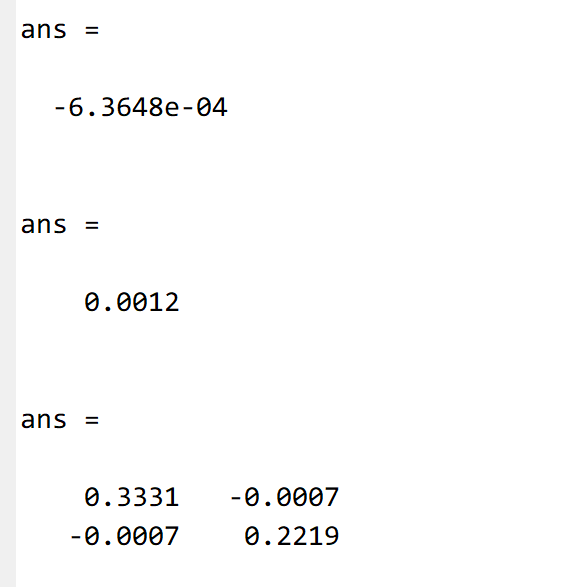
\includegraphics[width=0.9\linewidth]{./figure/task1_2a.png}
        \caption{第一种方法生成的均值和协方差矩阵}
    \end{subfigure}
    \begin{subfigure}{0.45\textwidth}
        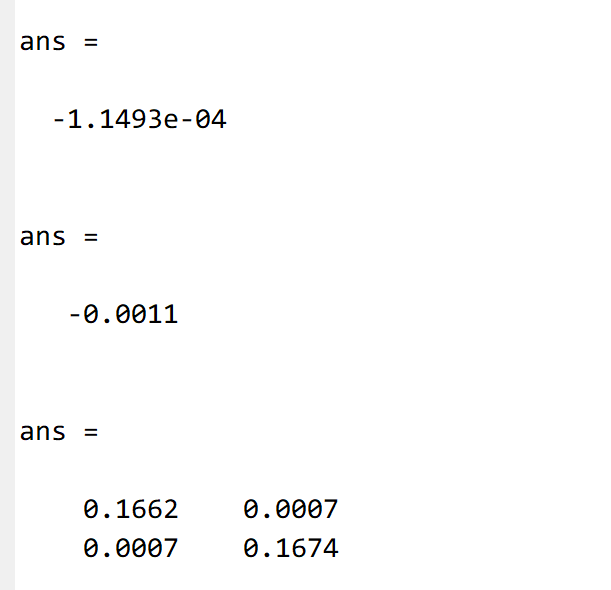
\includegraphics[width=0.9\linewidth]{./figure/task1_2b.png}
        \caption{第二种方法生成的均值和协方差矩阵}
    \end{subfigure}

    \caption{两种方法生成的均值和协方差矩阵}
\end{figure}

可以看出 $x$ 的均值基本为0,而 $y$ 基本接近0,但是协方差矩阵算出的值与理论值相距甚远,特别是第一行第一列和第二行第二列。
即他们不符合在单位圆上的均匀分布。

其次,画出图像也可以检验是否是均匀分布。
因为100,000个点太过于密集,所以画图取的样本数量为20,000个。
图像如下。
\begin{figure}[h!]

    \begin{subfigure}[h!]{0.45\textwidth}
        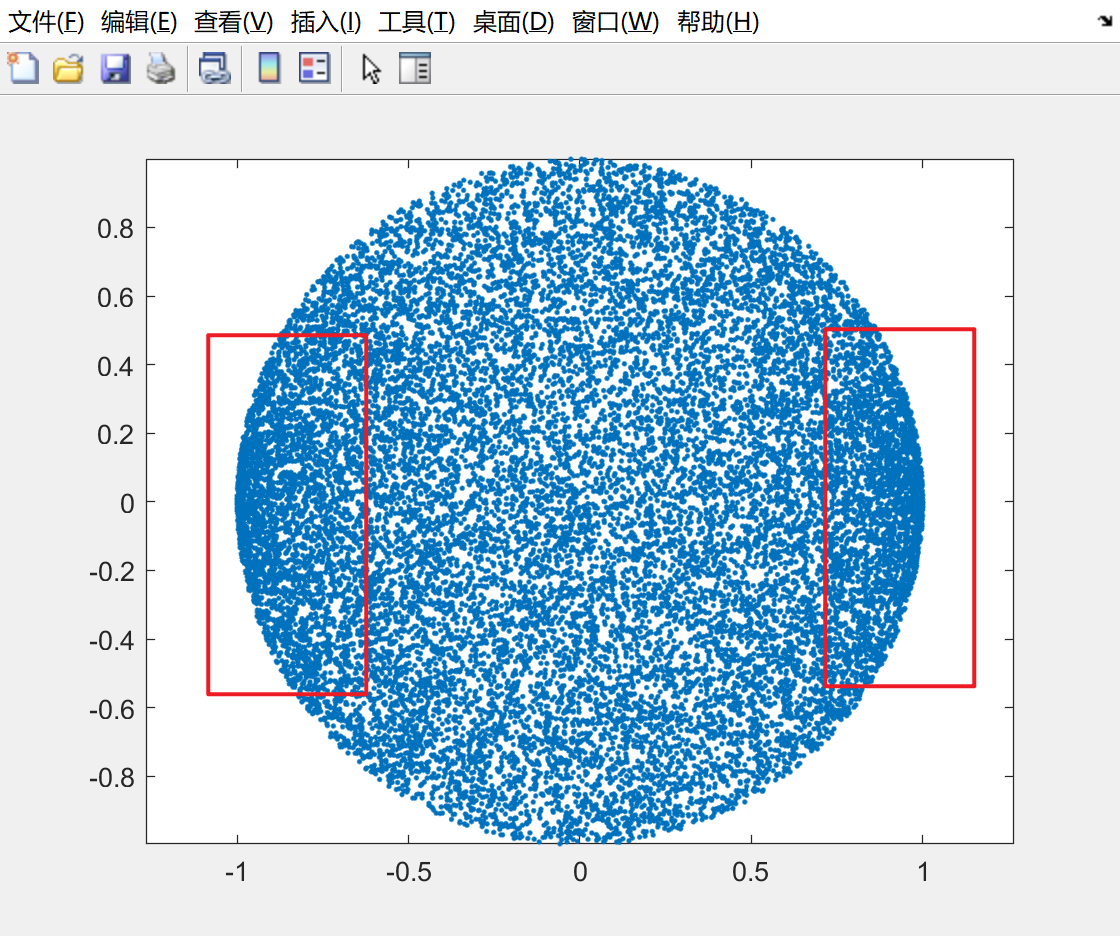
\includegraphics[width=0.9\linewidth]{./figure/task1_3a.png}
        \caption{第一种方法生成散点图}
    \end{subfigure}
    \begin{subfigure}[h!]{0.45\textwidth}
        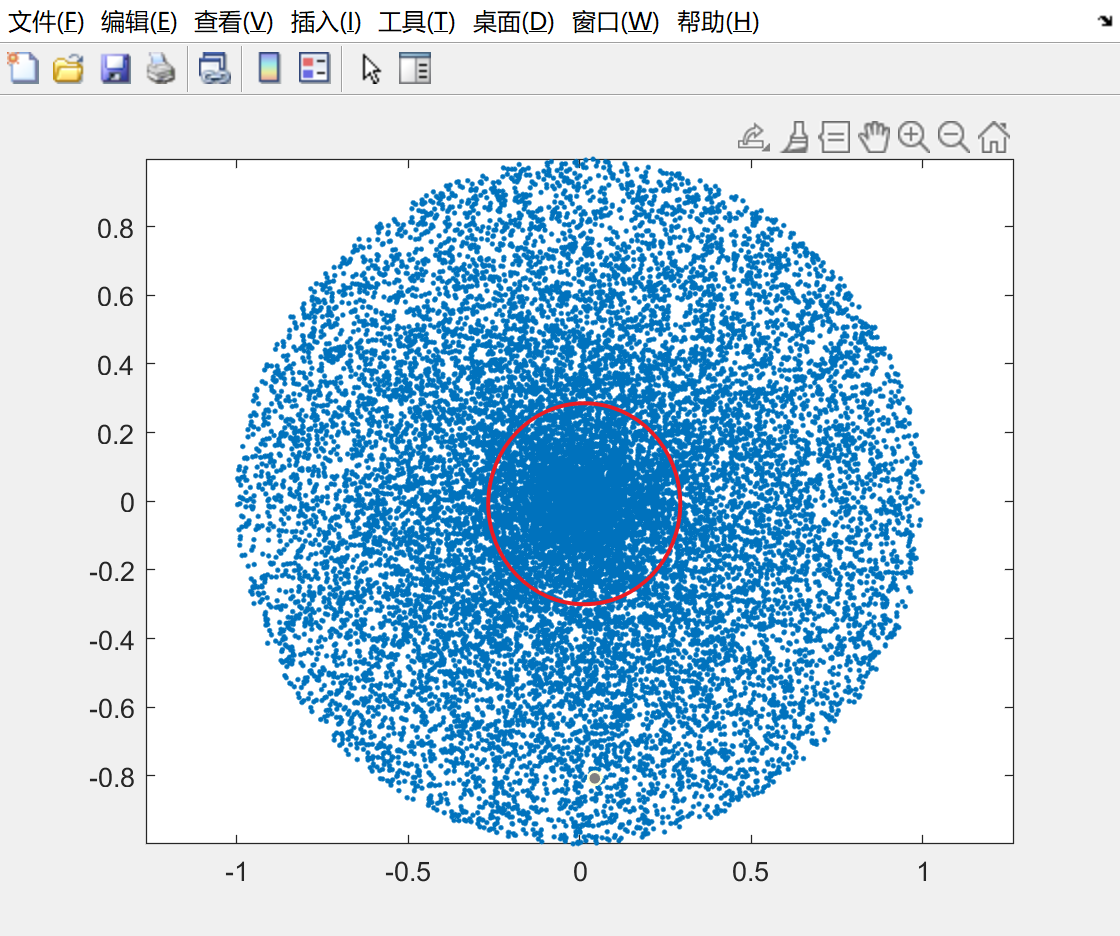
\includegraphics[width=0.9\linewidth]{./figure/task1_3b.png}
        \caption{第二种方法生成的散点图}
    \end{subfigure}

    \caption{两种方法生成的散点图}
\end{figure}

从上图中可以看出(用红色方框和红色园标注的地方),第一种情况下位于x轴的两端的点相比于其他部分更加密集。
而第二种情况下,越靠近x轴的区域分布越为密集。
因此,两种情况所生成的点坐标均不符合均匀分布。

\subsection{问题 2}

首先生成两个在 $[-1,1]$ 上的随机变量,并取这两个随机变量的平方和小于等于1.这样便生成了单位圆上的随机均匀分布。

按照上述步骤依次取三个点,可以分别记为 A,B,C,则可以算出 $\vec{AB}\ \&\ \vec{AC}$,
这样便可以算出 $\angle BAC$ 的余弦值,进而可以算出其正弦值,
因此可以用公式 $S_{\triangle ABC} =\frac12 |AB||AC|\sin\angle BAC$ 算出面积。

重复100000次,取平均值算出期望。代码如下
\lstinputlisting[language=Matlab]{task1_2_1.m}
算出的结果如图所示。

\begin{figure}[h!]
    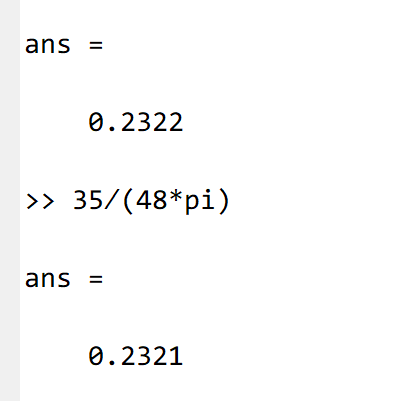
\includegraphics[width=0.4\linewidth]{./figure/task2_1.png}
    \caption{实验结果}
\end{figure}

可以看出用蒙特卡洛进行的实验和真实值非常接近,也就是小明的猜想是合理的。

下面来证明上述猜想。

首先,固定一个点 $C$ 在 $(0,1)$ ,在这个点时的期望三角形的面积的期望设为 $s$ 。

再令 $M=\max\{|OA|,|OB|,|OC|\}$ ,则我们所要求的期望则是
\[\mathbb{E}(A)=\int_{0}^{1} \mathbb{E}(A \mid M=r) \times 6 r^{5} d r=\int_{0}^{1} s r^{2}
    \times 6 r^{5} d r=\frac{3s}{4}\]
之后,我们便需要求出 $s$ 。

具体思路为:此时考虑原点在 $(0,1)$ 的情况,让 $C$ 在原点,则
$\angle ACx,\angle BCx \in (-\frac \pi2,\frac \pi2)$ ,分别记 $\angle ACx$ 和 $\angle BCx$ 为 $\phi,\psi$ 。
也不妨设$\phi \le \psi  \le \frac \pi2$,并最后乘以2即可。
\[\mathbb{E}_{1}=\frac{2}{\pi^{2}} \int_{-\pi/2}^{\pi/2} d \phi \int_{\phi}^{\pi/2} d \psi \int_{0}^{2 \sin \phi} d r \int_{0}^{2 \sin \psi} d s\left(\frac{1}{2} r s \sin (\psi-\phi) r s\right)\]

\vspace{1em}
最后算出 $s=\frac{35}{36\pi}$ ,则 $\mathbb{E}(A)=\frac{35}{48\pi}$ .

由此,可以设计出计算$\pi$的随机模拟实验。
取多次实验中的三角形面积取平均值,记为 $s$ ,之后计算 $\pi=\frac{35}{48s}$ .
设计的动画的代码如下(因为取值太大,动画时间太长,因此只取了前1000个进行实验)

\lstinputlisting[language=Matlab]{task1_2_2.m}

动画过程中的截图如下

\begin{figure}[h!]
    \begin{subfigure}[h!]{0.4\textwidth}
        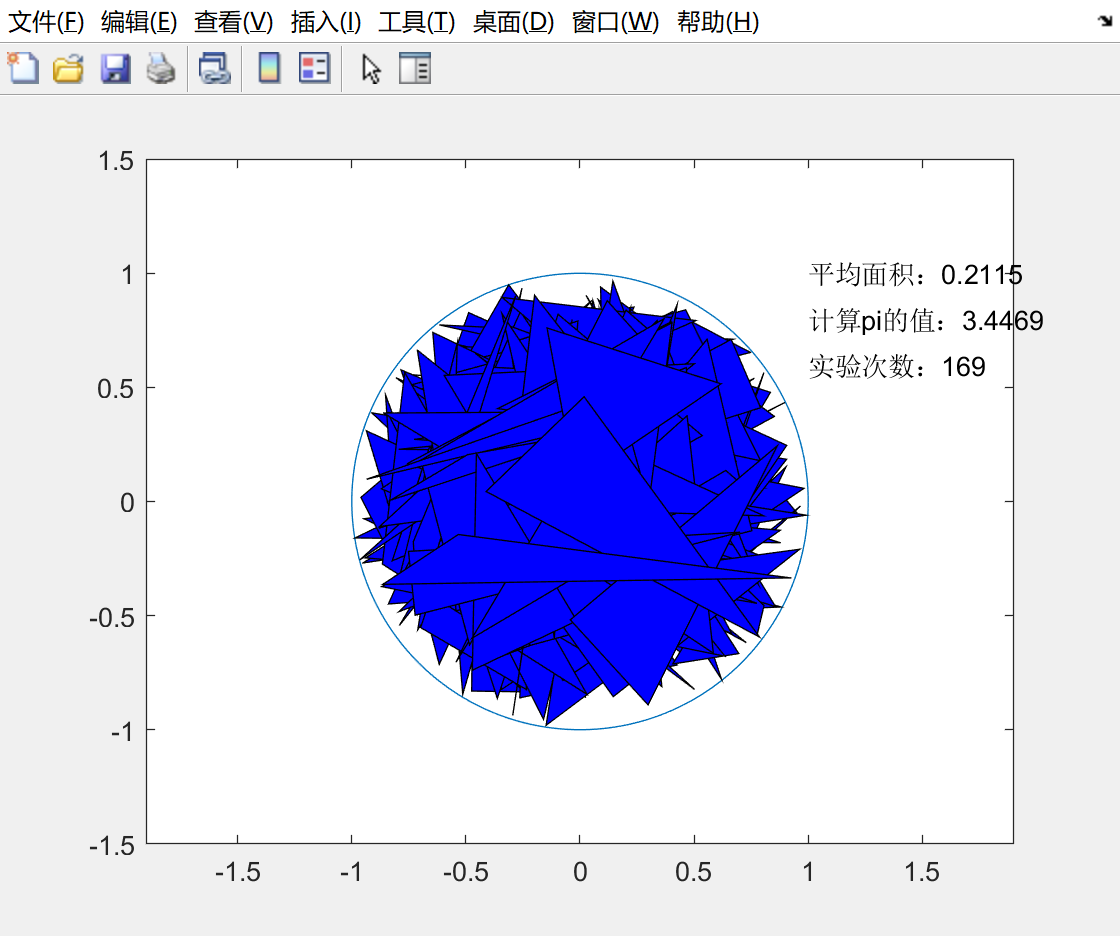
\includegraphics[width=0.9\linewidth]{./figure/task2_2.png}
        \caption{模拟实验前期}
    \end{subfigure}
    \begin{subfigure}[h!]{0.5\textwidth}
        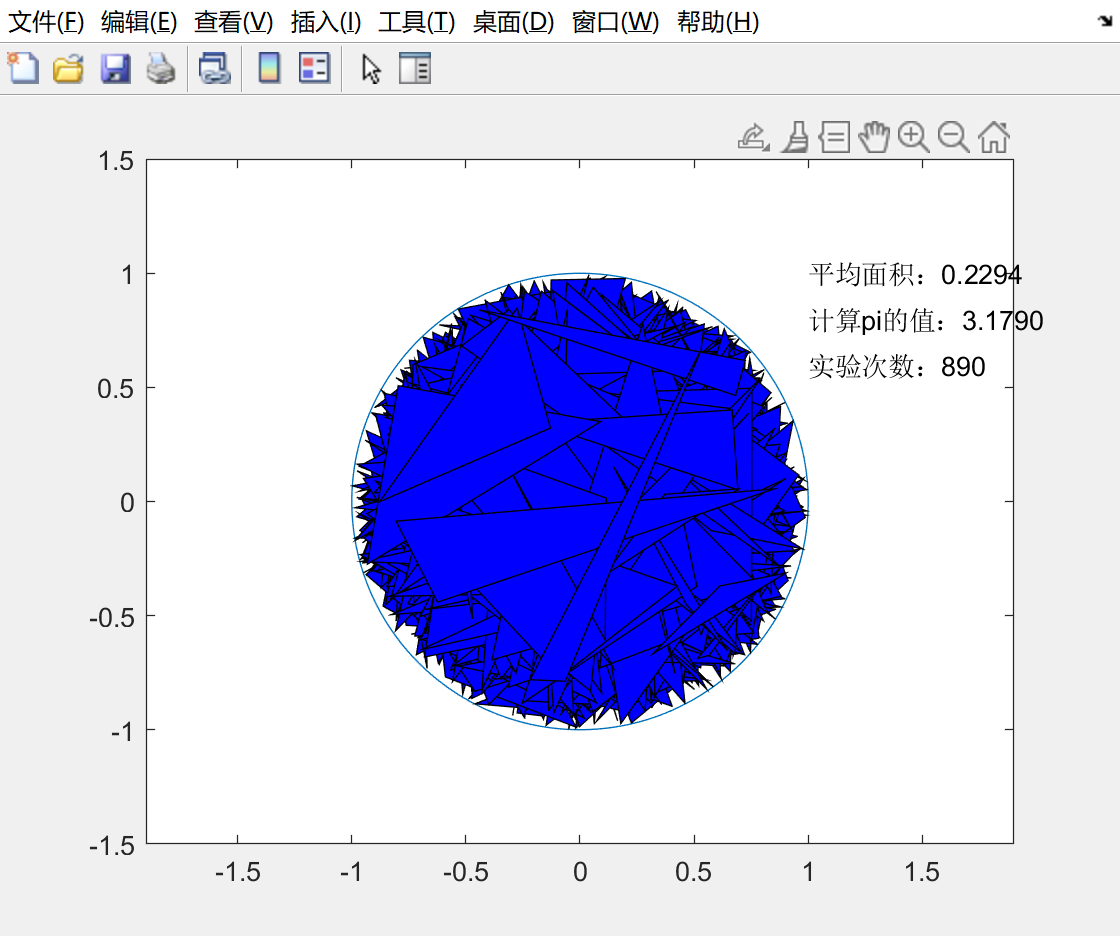
\includegraphics[width=0.9\linewidth]{./figure/task2_2b.png}
        \caption{模拟实验后期}
    \end{subfigure}
\end{figure}
可以看到随着实验次数的增加,算出的值越来越接近 $\pi$.

\section{探索性实验}

\subsection{问题 1}
首先借助在课上的内容,先生成 $D,m,E $三个变量,再在函数内部继续生成 $\tilde{D},\tilde{m}, \tilde{E}$
代码如下。

\lstinputlisting[language=Matlab]{task2_1_func.m}

之后再在程序中模拟实验,当不满足条件时,计数就会加一。
因此理想的情况下,计数应该为0.
代码如下。

\lstinputlisting[language=Matlab]{task2_1.m}

最后的输出结果则是0(因为图片只有一个0的答案,所以就没有贴图了),这也就说明该不等式是成立的。
下面来证明此不等式。
首先注意到 $\tilde{D},\tilde{m}$ 项都包含了 $1+tv$ 项,因此我们也想在 $E$ 中凑出 $1+tv$ 项。
由此
\[\tilde{E}=E+tm=\frac{\rho+C p}{1-v^{2}}-p+(\frac{\rho+C p}{1-v^{2}})t=\frac{(1+tv)(\rho+C p)}{1-v^{2}}-p
    =(E+p)(1+tv)-p=E(1+tv)+ptv\]
此时,计算 $\tilde{E}^2-(\tilde{D}^2+\tilde{m}^2)$ 是否大于0即可,而因为 $E^2>D^2+m^2$ ,因此只用计算式中一部份量即可。
计算得出的剩余量为
\[2(1+tv)(Ev-m)+tp(v^2-1)\]
此时,将这些值带入matlab中用符号向量计算化简可得 $p(tv^2+2v+t)$,又注意到此时 $t,v$ 的范围在 $[-1,1]$ 之间,则经过简单计算便可知该式大于0.
因此得证。

\subsection{问题 2}
首先生成一个符号变量 $x$,之后写出要解的方程的表达式,并用solve解出实根,观察是否只有一个实根,且这个实根是否大于0。
如果其中一个不满足的话则可以在计数器上加一。
而我们最终的期望的结果是0.
代码如下。

\lstinputlisting[language=Matlab]{task2_2.m}

得出的最终的结果也是0.
这也就是说从数学实验的角度证明这有一个唯一正解。
下面用理论的方式验证这个式子。

首先可以令
\[f(x)=Cx+\frac{m^2}{E+x}+D\sqrt {1-\frac{m^2}{(E+x)^2}}-E-x\]
注意到,当 $x\rightarrow \infty$ 时,$f(x)\rightarrow\infty$.
我们此时只要证明 \(f(x)\) 在 \((0,\infty)\) 上单调递增且 \(f(0)<0\) 即可。
而
\[f'(x)=C-1-\frac{m^2}{(E+x)^2} +\frac{2m^2}{ (E+x)^3 D/\sqrt {1-\frac{m^2}{ (E+x)^2 }}}=
    (C-1)+\frac{m^2}{(E+x)^2}(\frac{2D}{\sqrt {(E+x)^2-m^2}}-1)\]
先看后面部分:
\[\frac{2D}{\sqrt {(E+x)^2-m^2}} -1=\frac{2D}{\sqrt {E^2+2Ex+x^2-m^2}}-1<
    \frac{2D}{\sqrt {2Ex+x^2+D^2}}-1<\frac{2D}{\sqrt {D^2}}-1<1\]
同时,
\[\frac{2D}{\sqrt {(E+x)^2-m^2}} -1 \geq -1\]
而由不等式 \(E>\sqrt {D^2+m^2}\)得
\[\frac{m^2}{(E+x)^2}<1\]
因此,后半部分的范围必在 $[-1,1]$.
又 $C-1>1$, 因此, $f'(x)\geq 0$ 在 $(0,\infty)$ 上成立。

之后再证明 $f(0)<0$ 即可。
\[f(0)=\frac{m^2}{E}+D\sqrt {1-\frac{m^2}{E^2}}-E=\frac{(m^2-E^2)+D\sqrt {E^2-m^2}}{E}\]
把 \(\sqrt {E^2-m^2}\) 当作自变量,且取值范围为 $(D,\infty)$,此时分母是一个二次函数,因此易得此时这个值是小于0的。

综上,该方程式有唯一的正实根。

下面是编写的程序
\lstinputlisting[language=Matlab]{task2_2_func.m}


\subsection{问题 3}
在上一问的基础上将 $x=p$ 代入,并检测左式减去右式的绝对值是否小于机器误差,如果满足则可以认为该值等于0,记满足等式。
得出0则计数器加一,最后理应得到跟循环次数相等的值。
代码如下。
\lstinputlisting[language=Matlab]{task2_3.m}
最后得出的值为100000,因此这个等式是成立的。

\subsection{问题 4}
结合问题2\textasciitilde3,可以得出满足(2)的方程有且只有唯一的正实根,且该根为 $p$
因此,据此可以解出 $p$,且由唯一性可知,这正是生成 $D,m,E$ 所用的 $p$

又注意到 $E=\frac{m}{v}-p$,而此时 $E,m,p$ 都是已知的,因此可以求出 $v$.
将求出的 $v$ 代入到 $D$ 中就可以得出 $\rho$.
因此对于任意的 $(D, m, E) \in A$ ,都可以找出一组唯一的 $(\rho,p,v)$ 。

因此,这个多元向量函数值是双射。


\end{document}